\section{Web前端实现}

OJ系统中前端页面主要分为两部分,用户前台和admin后台,两部分应用场景有着明显的差异。用户前台,逻辑简单,主要以展示为主,需要兼顾搜索引擎的抓取;admin后台,界面逻辑非常复杂,有大量的列表页、动态验证项目、动态变化的表单,不需要考虑搜索引擎的抓取问题。需要进行实际的分析,选择不同的开发技术。

\subsection{admin后台的SPA页面实现}

\subsubsection{JavaScript模块化}

页面功能的复杂化往往伴随的是JavaScript代码的数量的爆炸,传统的使用\texttt{script}标签直接加载的方案会遇到很多问题,比如无法确定模块依赖顺序、文件合并复杂等。由于历史原因,JavaScript 并未提供一种原生的、语言级别的模块化组织模式,而是将模块化的方法交由开发者来实现。因此,出现了很多种 JavaScript 模块化的实现方式,比如,CommonJS Modules、AMD 等。我们使用了AMD的模块化方案,由require.js充当加载器\cite{js-module}。

\begin{verbatim}
define("bsAlert", ["jquery", "bootstrap"], function($){
     function bsAlert(content){
         // TODO
     }
    return bsAlert;
});
\end{verbatim}

\texttt{bsAlert}是模块名,\texttt{jquery}和\texttt{bootstrap}是模块的依赖,加载\texttt{bsAlert}模块的时候,require.js会自动去加载它的依赖模块。

使用\texttt{require}函数引用这个模块,获得函数引用。

\begin{verbatim}
require(["bsAlert"], function (bsAlert) {
    bsAlert("foobar");
})
\end{verbatim}

同时,由于已经确定模块间依赖关系,r.js可以将模块级别和页面级别的JavaScript合并成一个文件,这样就减少了页面上的网络请求次数,提高了性能和用户体验。以admin后台添加题目为例:

\begin{table}[H]
\centering  % 表居中
\caption{合并JavaScript前后网络请求统计}
\begin{tabular}{|c|c|c|}  % {lccc} 表示各列元素对齐方式,left-l,right-r,center-c
\hline
是否合并 &网络请求次数 &网络请求数据量\\ \hline  % \hline 在此行下面画一横线
否 &43 &1.3M\\         % \\ 表示重新开始一行
\hline
是 &15 &844K\\
\hline
\end{tabular}
\end{table}

\subsubsection{MVVM框架}

在传统前端开发中,大量的动态效果需要直接进行DOM操作和拼接HTML操作,这是造成JavaScript代码无法维护的元凶之一,使用MVVM框架可以不再手动操作DOM,简化了操作,而且可以提高性能。OJ系统使用的是avalon.js框架,类似的框架还有 Vue.js和Angular JS。

所有前端代码彻底分成两部分,视图的处理通过绑定实现,业务逻辑则集中在VM对象中处理。我们只要操作VM的数据,它就自动的同步到视图。demo如下:

\begin{verbatim}
<script>
var vm = avalon.define({
    $id: "demo",
    name: "foobar"
})
</script>

<body ms-controller="demo">
    <input ms-duplex="name">
    <p>Hello,{{name}}!</p>
</body>
\end{verbatim}

这样页面加载的时候,文本框和"hello"后面中就会显示"foobar",然后随着用户修改文本框中的文字,页面上"hello"后面的文字也会自动改变。

\subsubsection{Web组件}
前端开发的时候经常会遇到一些重复的功能和逻辑,比如翻页模块、上传模块、富文本编辑器等,将底层的UI组件与自己的业务逻辑联系在一起然后复用才能提高开发效率,增强代码的可维护性。admin后台有多个封装的Web组件,以翻页pager组件为例。

\begin{verbatim}
avalon.component("ms:pager", {
    $template: "页数: {{ currentPage }}/{{ totalPage }} " +
    "<button ms-class=\"{{ currentPage==1?'btn disabled':'btn' }}
    \"ms-click=\"_getPrevPage\">上一页</button> " +
    " <button ms-class=\"{{ currentPage==totalPage?'btn disabled':'btn' }}
    \" ms-click=\"_getNextPage\">下一页</button>",
    currentPage: 1,
    totalPage: 1,
    _getPrevPage: _interface,
    _getNextPage: _interface,
    $init: function (vm, el) {
        vm._getPrevPage = function () {
            if (vm.currentPage > 1) {
                vm.currentPage--;
                vm.getPage(vm.currentPage);
            }
        };
        vm._getNextPage = function () {
            if (vm.currentPage < vm.totalPage) {
                vm.currentPage++;
                vm.getPage(vm.currentPage);
            }
        };
    }
\end{verbatim}

在页面上只要使用
\begin{verbatim}
<ms:pager $id="userPager" config="pager"></ms:pager>
\end{verbatim}就可以得到有完整功能的翻页按钮,不需要每个页面都去重复代码,而且不需要关心内部实现。

\subsubsection{前后端分离}

我们在传统前端开发过程中有很多痛点:

\begin{itemize}
\item[-] 前端开发依赖后端,一般需要后端功能完成后,由后端向前端模板传递变量完成渲染,才能进行开发和测试,而且前端可能需要搭建后端开发环境。或者前端先完成一个demo页面,然后由后端工程师转换为实际的框架模板。
\item[-] 前端模板中有大量的后端语言逻辑,导致模板维护性变差。
\item[-] 前端模板数据更新需要刷新页面,而整个页面的完全加载是对带宽和性能的浪费。
\end{itemize}

由于网页前端越来越复杂,为了提升开发和测试效率,前后端分离的技术使用的越来越多,后端主要负责业务逻辑实现和提供API接口,前端负责构建页面和展示数据。

\subsubsection{admin后台整体框架}
由于admin后台是一个SPA页面,页面无刷新,URL不会变化,所以需要使用URL中的hash存储页面路由信息。比如\texttt{/admin/\#announcement/announcement}、\texttt{/admin/\#user/user\_list}等,JavaScript监听hash变化事件,修改\texttt{vm.templateUrl},加载不同的HTML模板。

\begin{verbatim}
<div ms-include-src="templateUrl" data-include-replace="true"></div>
\end{verbatim}

\begin{figure}[H]
\centering
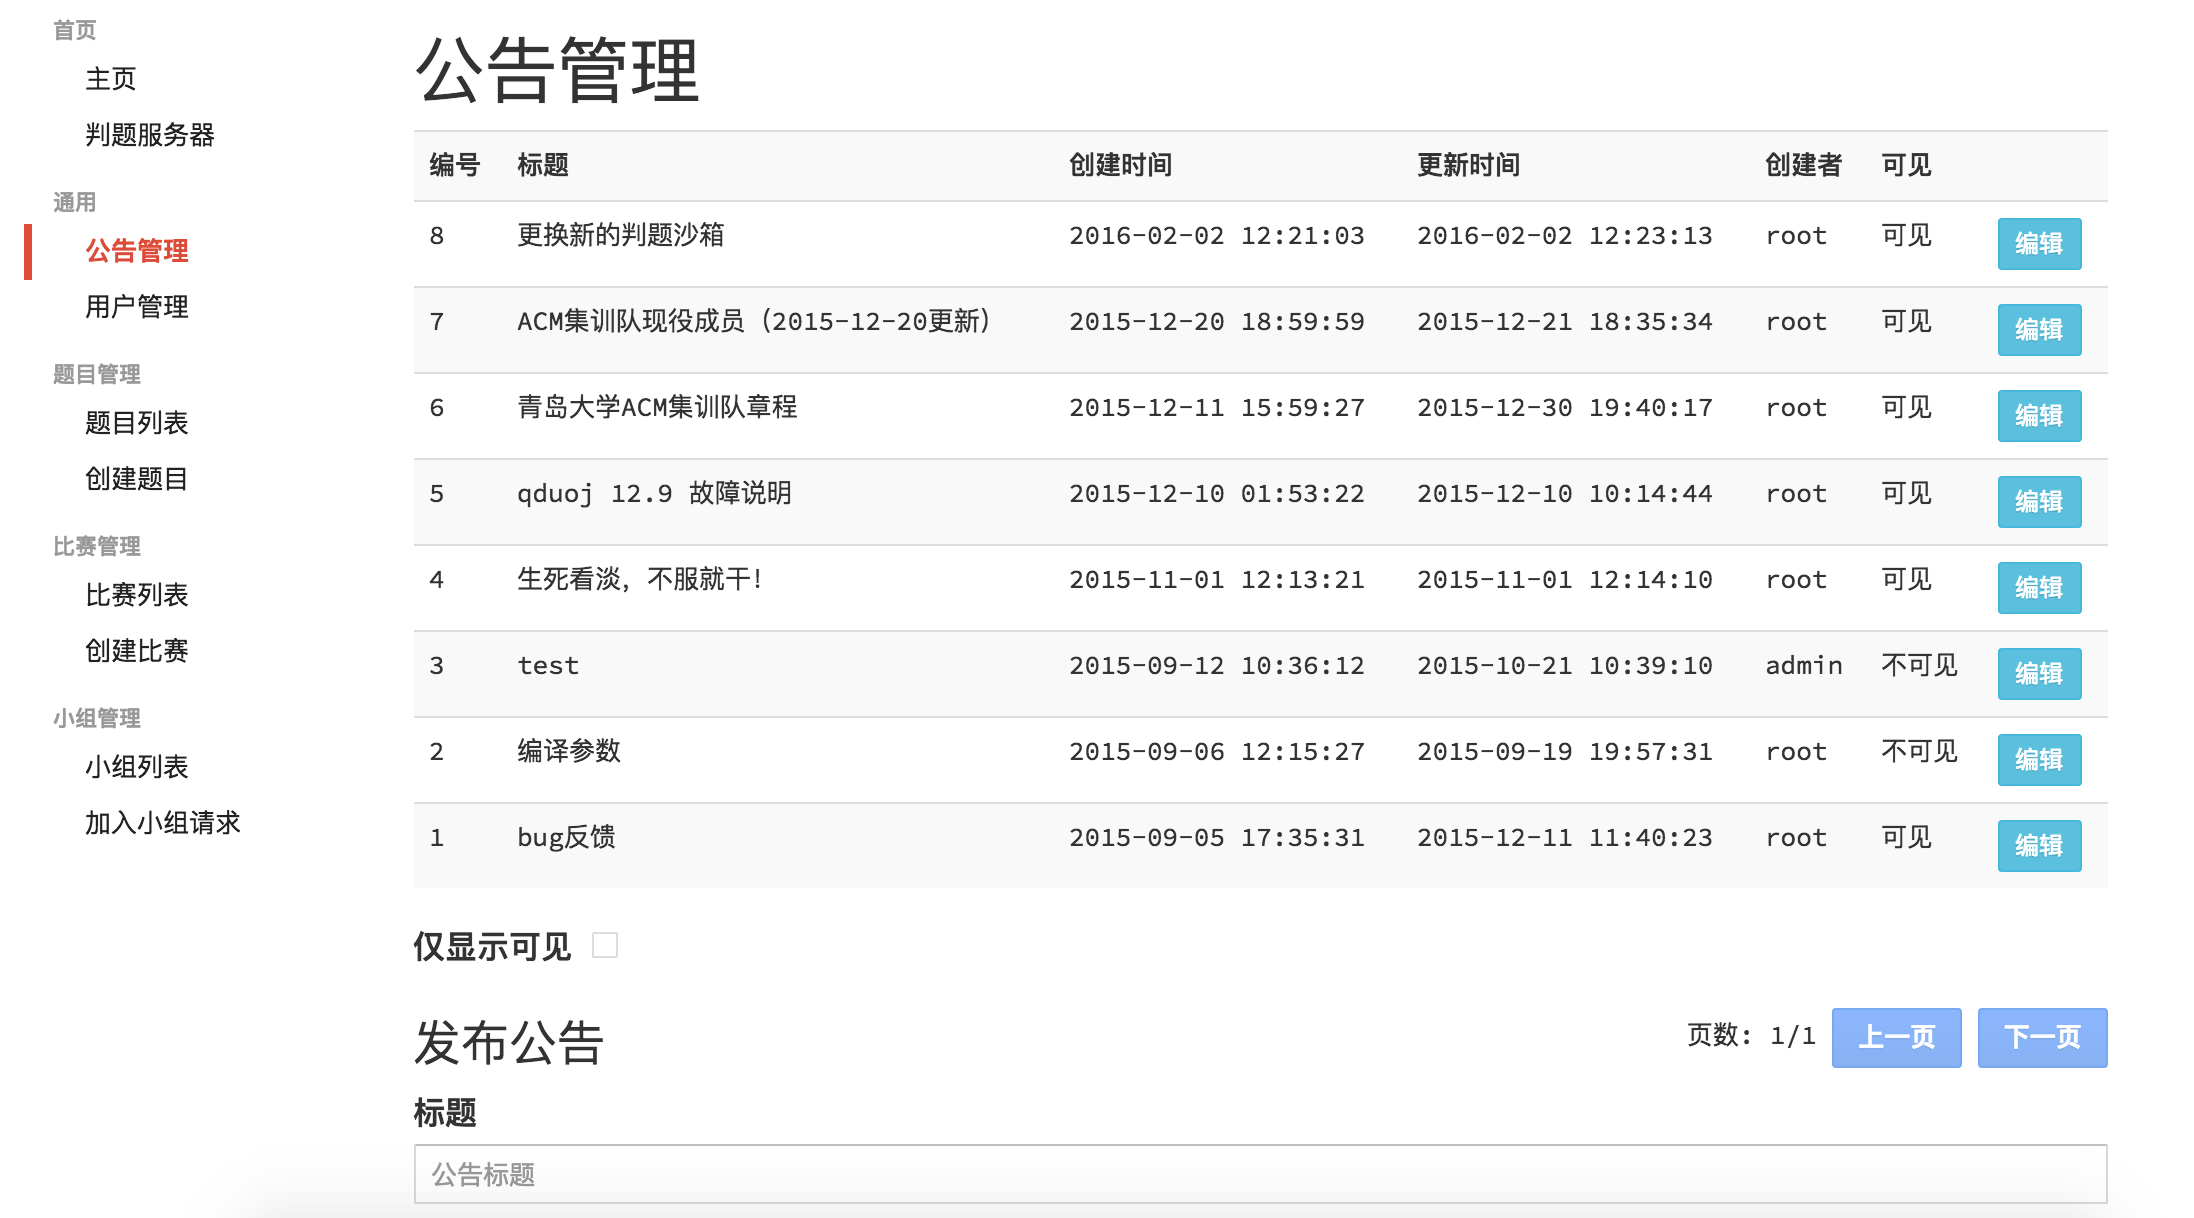
\includegraphics[width=0.9\textwidth]{admin-index}
\caption{admin首页}
\end{figure}

\subsubsection{用户管理页面的实现}
本节将以后台用户管理页面为例,解释admin模块前端开发的流程。

用户管理页面主要分为用户翻页列表和用户编辑两部分。对于用户列表,在VM中存储一个数组,然后在前端模板进行循环。

\begin{verbatim}
var vm = avalon.define({
    $id: "userList",
    userList: []
}
\end{verbatim}

HTML模板的部分代码

\begin{verbatim}
<tr ms-repeat="userList">
    <td>{{ el.id }}</td>
    <td>{{ el.username }}</td>
    <td>{{ el.create_time|date("yyyy-MM-dd HH:mm:ss")}}</td>
    <td>{{ el.real_name }}</td>
    <td>{{ el.email }}</td>
</tr>
\end{verbatim}

页面加载的时候,JavaScript通过ajax去后端查询分页用户列表,然后赋值给vm.userList,这时HTML模板中就会自动显示为列表项目。

\begin{verbatim}
function getPage(page) {
    var url = "/api/admin/user/?paging=true&page=" + page + "&page_size=10";
    $.ajax({
        beforeSend: csrfTokenHeader,
        url: url,
        dataType: "json",
        method: "get",
        success: function (data) {
            if (!data.code) {
                vm.userList = data.data.results;
                avalon.vmodels.userPager.totalPage = data.data.total_page;
            }
            else {
                bsAlert(data.data);
            }
        }
    });
}
\end{verbatim}

\begin{figure}[H]
\centering
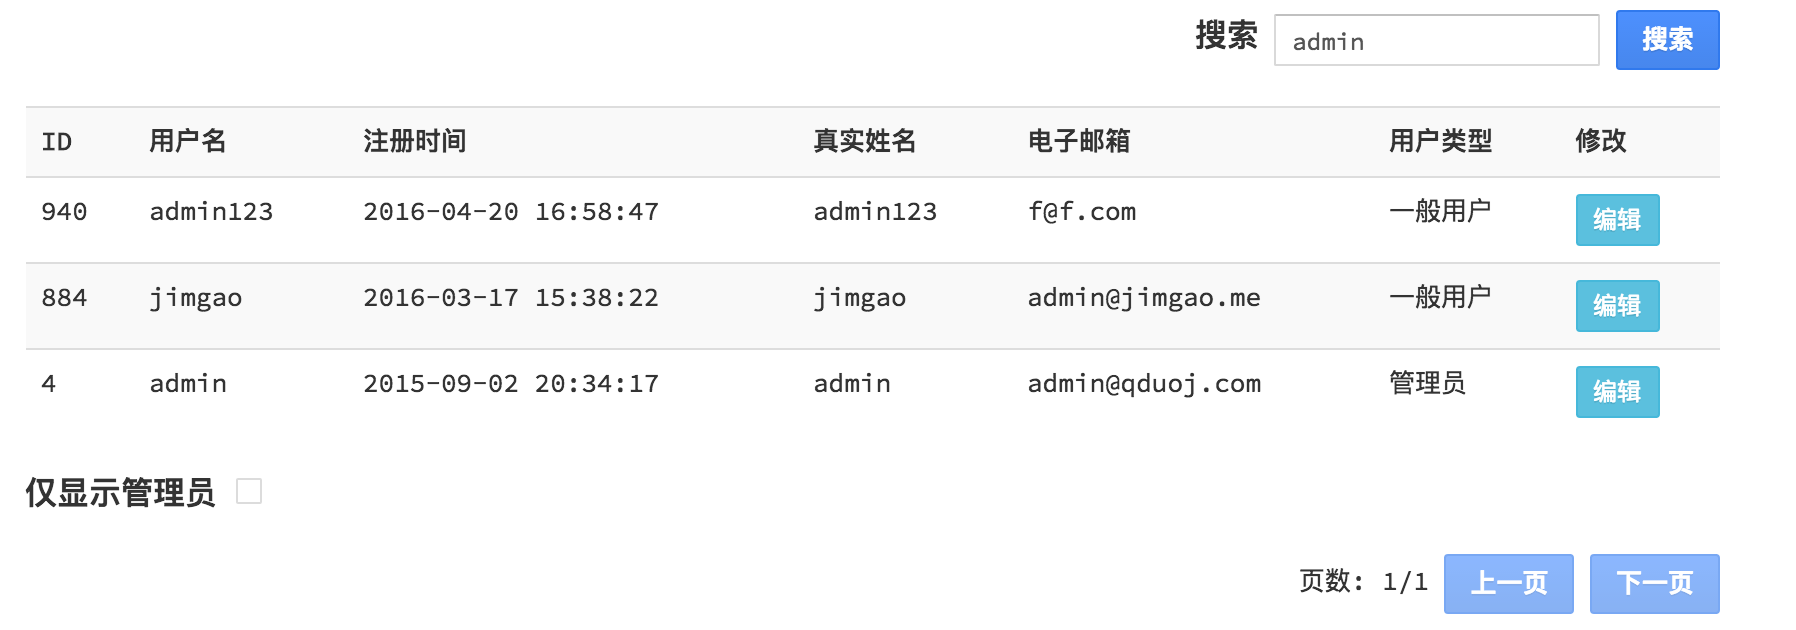
\includegraphics[width=0.9\textwidth]{admin-users}
\caption{admin用户列表}
\end{figure}

编辑用户的时候,需要VM中增加几个同步变量,比如\texttt{name}、\texttt{email}等,然后与input双向绑定。以用户名为例。

\begin{verbatim}
<div class="form-group col-md-4"><label>用户名</label>
    <input type="text" class="form-control" ms-duplex="username"
           data-minlength="3" data-minlength-error="用户名不得少于3位" required>
    <div class="help-block with-errors"></div>
</div>
\end{verbatim}

vm.username的修改将导致页面显示的修改,用户输入用户名将导致vm.username的修改。

最后通过AJAX请求后端更新用户信息

\begin{verbatim}
$("#edit-user-form").validator()
.on('submit', function (e) {
    if (!e.isDefaultPrevented()) {
        var data = {
            username: vm.username,
            email: vm.email,
            // 省略部分属性
        };
        $.ajax({
            url: "/api/admin/user/",
            data: data,
            dataType: "json",
            method: "put",
            success: function (data) {
                if (!data.code) {
                    bsAlert("编辑成功!");
                    getPage(1);
                } else {
                    bsAlert(data.data);
                }
            }
        });
        return false;
    }
});
\end{verbatim}

\begin{figure}[H]
\centering
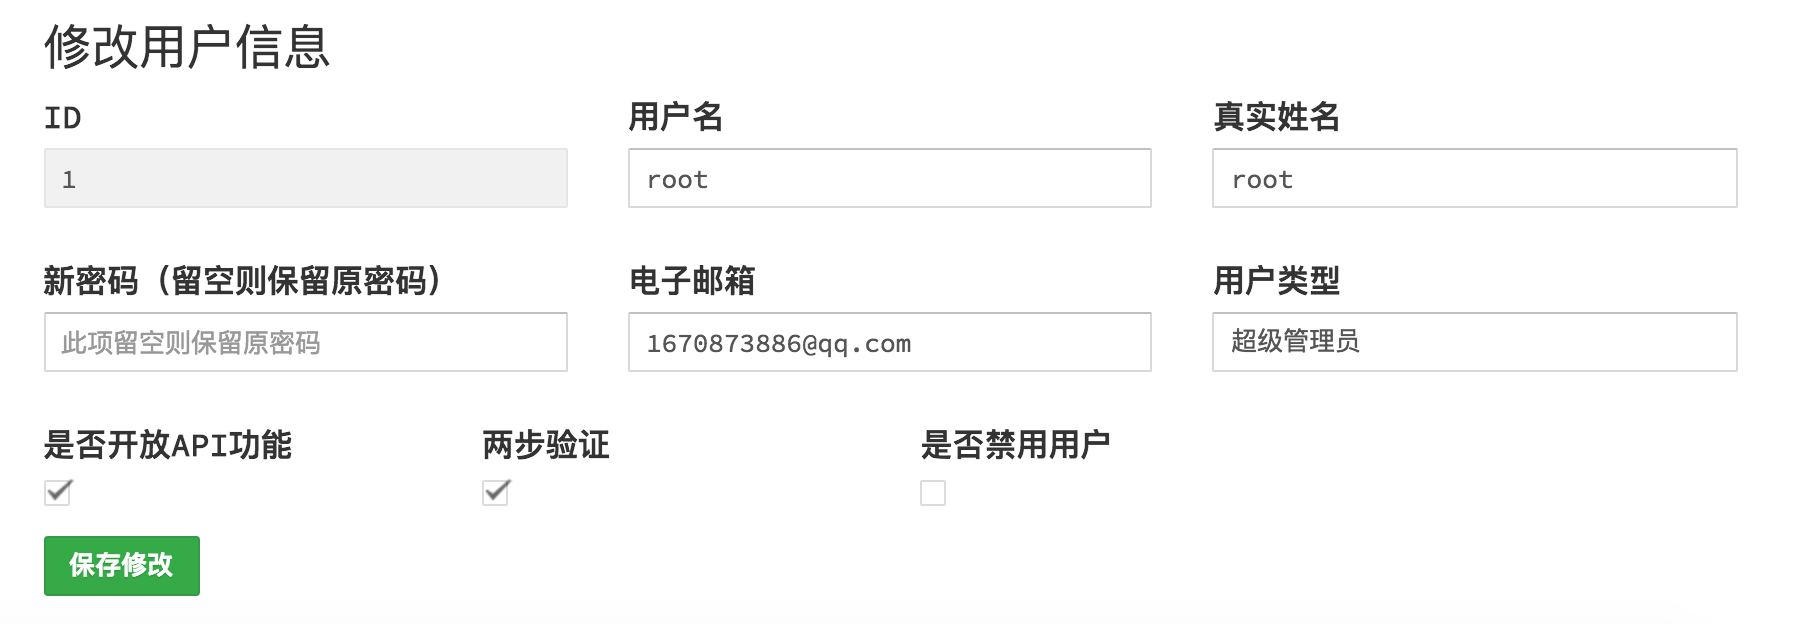
\includegraphics[width=0.9\textwidth]{admin-edit-user}
\caption{admin编辑用户}
\end{figure}

在更加复杂的页面上也是类似的思路,只是使用了更多的绑定、Web组件和更加复杂的业务逻辑和动态效果。

\subsection{用户前台的后端渲染页面}

和前后端分离然后前端渲染页面相比较,后端渲染要简单的多,也是最传统的做法。因为Django是MVC的架构,我们View中的逻辑去Model中查询,然后传递给模板就可以了。模板中变量占位符将渲染为实际的值,还可以使用简单的逻辑判断,还可以调用函数。

以题目详情页为例:

\begin{verbatim}
def problem_page(request, problem_id):
    try:
        problem = Problem.objects.get(id=problem_id, visible=True)
    except Problem.DoesNotExist:
        return error_page(request, u"题目不存在")
    return render(request, "oj/problem/problem.html", {"problem": problem})
\end{verbatim}

部分模板的代码

\begin{verbatim}
<div class="problem-section">
    <label class="problem-label">描述</label>
    <div class="problem-detail">{{ problem.description|safe }}</div>
</div>
<div class="problem-section">
    <label class="problem-label">输入</label>
    <p class="problem-detail">{{ problem.input_description }}</p>
</div>
\end{verbatim}